\documentclass[a4paper,11pt]{article}
\usepackage{ctex}
\usepackage{enumerate}
\usepackage{times}
\usepackage{mathptmx}
\usepackage{amsmath}
\usepackage{amssymb}
\usepackage{array}
\usepackage{tikz}
\usepackage[top=2cm, bottom=2cm, left=2cm, right=2cm]{geometry}

%\allowdisplaybreaks[4]
\renewcommand{\labelenumi}{\textbf{\emph{\alph{enumi}}.}}
\begin{document}
  \title{����~2-4~��ҵ}
  \author{��������ۿԴ \and ѧ�ţ�161240004}
  \date{}
  \maketitle

  \section{[CS] Problem 4.1-16}
  Failure occurs in inductive step. If we don't specify that the ears are nonadjacent, it is possible that two ears are connected by an edge. When rejoining two polygons into a larger one along the diagonal, the two ears of each polygons might be both incident to the diagonal, and they are eliminated once joined. Thus there is no ear in the new polygon, and we fail to complete the proof.

  \section{[CS] Problem 4.1-17}
  The relationship between the number of vertices in a polygon ($V$) and the number of triangles in any triangulation of tat polygon ($N$) is $V=N-2$. \par
  The base case is that the polygon is a triangle. In this case, $V=3$, $N=1$, so the relationship holds. \par
  For every triangulated polygon, denoted by $A$, if it is not a triangle, then it must have at least diagonal. Split the polygon into two smaller polygons, denoted by $B$ and $C$, and we have $V_B = N_B - 2$, $V_C = N_C - 2$. Then rejoin the two diagonals along the diagonal. Obviously we get $N_A = N_B + N_C$. When rejoining, two edges coincide to form the diagonal, so $N_C = V_B + V_C - 2 = N_B - 2 + N_C - 2 + 2 = N_A - 2$. Therefore, the relationship holds for the larger polygon. \par
  By structural induction, we have proved that the relationship $V=N-2$ holds for all polygons.

  \section{[CS] Problem 4.2-8}
  Assume the number of fish in the lake after $n$ years is $T(n)$, then the recurrence is $T(n) = 2T(n-1) + 2000$. \par
  This recurrence is a first-order linear recurrence. Apply Theorem 4.5, we obtain
  \begin{align*}
    T(n) &= 2^n T(0) + \sum_{i=1}^n 2^{n-i} \times 2000 \\
    &= 2^n T(0) + 2000 \sum_{i=0}^{n-1} 2^i \\
    &= 2^n T(0) + 2000(2^n-1)
  \end{align*}

  \section{[CS] Problem 4.2-11}
  Apply Theorem 4.5,
  \begin{align*}
    T(n) &= 2^n T(0) + \sum_{i=1}^n 2^{n-i} i2^i \\
    &= 2^n + \sum_{i=1}^n i 2^n \\
    &= 2^n + 2^n \frac{n(n+1)}{2}
  \end{align*}

  \section{[CS] Problem 4.2-17}
  Apply Theorem 4.5,
  \begin{align*}
    T(n) &= r^n T(0) + \sum_{i=1}^n r^{n-i}i \\
    &= r^n + \sum_{i=1}^n i r^{n-i} \\
  \end{align*}
  Now we have to calculate $\sum_{i=1}^n i r^{n-i}$. Let $S(n)$ denote $\sum_{i=1}^n i r^{n-i}$, then we have
  \begin{align}
    S(n) &=  \qquad\quad\;\; 1 \times r^{n-1}  + \cdots + (n-1) \times r^1 + n \times r^0 \\
    rS(n) &= 1 \times r^n +  2 \times r^{n-1} + \cdots + n \times r^1
  \end{align}
  Subtracting (1) from (2), we obtain
  \begin{align*}
    (r-1)S(n) &= \sum_{i=1}^{n} r^i - n \\
    &= \frac{r^{n+1}-r}{r-1} - n
  \end{align*}
  Since $r \neq 1$, dividing both sides by $(r-1)$ yields
  $$ S(n) = \frac{r^{n+1}-r-nr+n}{(r-1)^2} $$
  Therefore
  $$ T(n) = r^n + \frac{r^{n+1}-r-nr+n}{(r-1)^2} $$

  \section{[CS] Problem 4.3-9}
  \begin{enumerate}
    \item Recursion tree: \\[0.2cm]
    \scriptsize
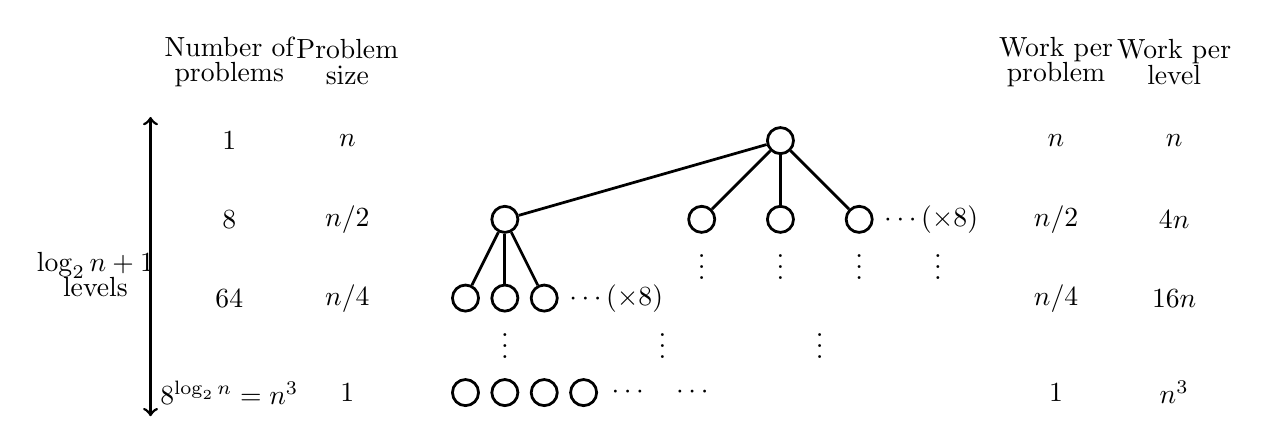
\begin{tikzpicture}[line width = 1pt,
                    solid/.style = {circle, draw, fill = black, minimum size = 0.3cm},
                    empty/.style = {circle, draw, fill = white, minimum size = 0.3cm}]

\draw[<->] (-2, 0.3) -- (-2, -3.5);
\node at (-2.7, -1.7)[align=center]{$\log_2 n + 1$ \\[-0.1cm] levels};

\node at (-1,1)[align=center]{Number of \\[-0.1cm] problems};
\node at (0.5,1)[align=center]{Problem \\[-0.1cm] size};

% number of problems
\node at (-1,0) {1};
\node at (-1,-1) {8};
\node at (-1,-2) {64};
\node at (-1,-3.2) {$8^{\log_2 n} = n^3$};

% problem size
\node at (0.5,0) {$n$};
\node at (0.5,-1) {$n/2$};
\node at (0.5,-2) {$n/4$};
\node at (0.5,-3.2) {1};

\node at (9.5,1)[align=center]{Work per \\[-0.1cm] problem};
\node at (11,1)[align=center]{Work per \\[-0.1cm] level};

% work per problem
\node at (9.5,0) {$n$};
\node at (9.5,-1) {$n/2$};
\node at (9.5,-2) {$n/4$};
\node at (9.5,-3.2) {1};

% work per level
\node at (11,0) {$n$};
\node at (11,-1) {$4n$};
\node at (11,-2) {$16n$};
\node at (11,-3.2) {$n^3$};

\node [empty] (T11) at (6,0) {};
\node [empty] (T21) at (2.5,-1) {};
\node [empty] (T22) at (5,-1) {};
\node [empty] (T23) at (6,-1) {};
\node [empty, label = right:$\cdots (\times 8)$] (T24) at (7,-1) {};
\node [empty] (T31) at (2,-2) {};
\node [empty] (T32) at (2.5,-2) {};
\node [empty, label = right:$\cdots (\times 8)$] (T33) at (3,-2) {};
\node at (5, -1.5) {$\vdots$};
\node at (6, -1.5) {$\vdots$};
\node at (7, -1.5) {$\vdots$};
\node at (8, -1.5) {$\vdots$};
\node at (2.5, -2.5) {$\vdots$};
\node at (4.5, -2.5) {$\vdots$};
\node at (6.5, -2.5) {$\vdots$};

\node [empty] at (2,-3.2) {};
\node [empty] at (2.5,-3.2) {};
\node [empty] at (3,-3.2) {};
\node [empty] at (3.5,-3.2) {};
\node at (4.5, -3.2) {$\cdots \quad \cdots$};

\draw (T11)--(T21);
\draw (T11)--(T22);
\draw (T11)--(T23);
\draw (T11)--(T24);
\draw (T21)--(T31);
\draw (T21)--(T32);
\draw (T21)--(T33);
\end{tikzpicture}\par
\normalsize
For the $i$-th level, the total work is $4^{i-1} n$. Summing over the levels, we get
\begin{align*}
  T(n) &= \sum_{i=1}^{\log_2 n + 1} 4^{i-1} n \\
  &= n \sum_{i=0}^{\log_2 n } 4^i \\
  &= n \frac{4^{\log_2 n + 1}  -1} {4-1} \\
  &= \frac{4}{3}n^3 - \frac{n}{3} \\
  &= \Theta(n^3)
\end{align*}

    \item Recursion tree: \\[0.2cm]
    \scriptsize
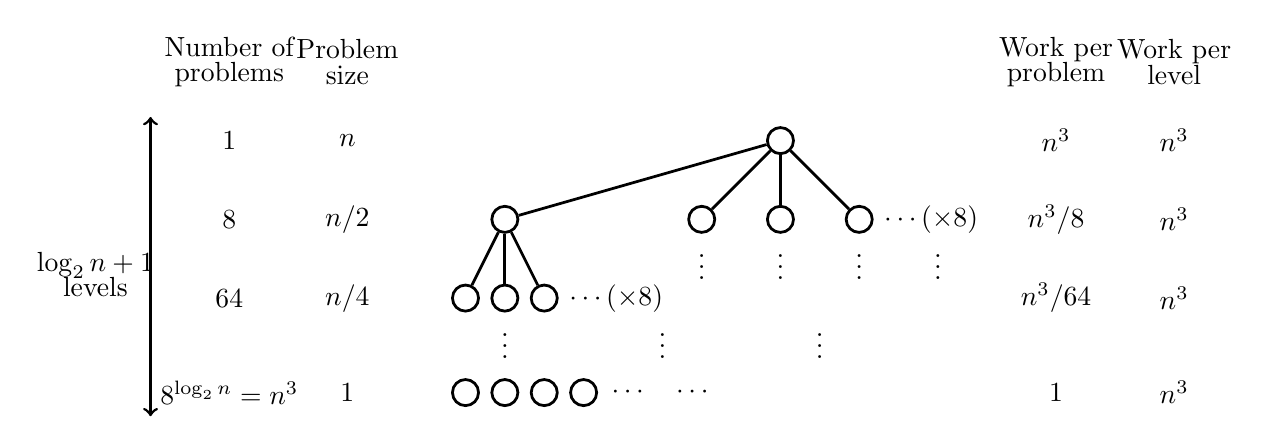
\begin{tikzpicture}[line width = 1pt,
                    solid/.style = {circle, draw, fill = black, minimum size = 0.3cm},
                    empty/.style = {circle, draw, fill = white, minimum size = 0.3cm}]

\draw[<->] (-2, 0.3) -- (-2, -3.5);
\node at (-2.7, -1.7)[align=center]{$\log_2 n + 1$ \\[-0.1cm] levels};

\node at (-1,1)[align=center]{Number of \\[-0.1cm] problems};
\node at (0.5,1)[align=center]{Problem \\[-0.1cm] size};

% number of problems
\node at (-1,0) {1};
\node at (-1,-1) {8};
\node at (-1,-2) {64};
\node at (-1,-3.2) {$8^{\log_2 n} = n^3$};

% problem size
\node at (0.5,0) {$n$};
\node at (0.5,-1) {$n/2$};
\node at (0.5,-2) {$n/4$};
\node at (0.5,-3.2) {1};

\node at (9.5,1)[align=center]{Work per \\[-0.1cm] problem};
\node at (11,1)[align=center]{Work per \\[-0.1cm] level};

% work per problem
\node at (9.5,0) {$n^3$};
\node at (9.5,-1) {$n^3/8$};
\node at (9.5,-2) {$n^3/64$};
\node at (9.5,-3.2) {1};

% work per level
\node at (11,0) {$n^3$};
\node at (11,-1) {$n^3$};
\node at (11,-2) {$n^3$};
\node at (11,-3.2) {$n^3$};

\node [empty] (T11) at (6,0) {};
\node [empty] (T21) at (2.5,-1) {};
\node [empty] (T22) at (5,-1) {};
\node [empty] (T23) at (6,-1) {};
\node [empty, label = right:$\cdots (\times 8)$] (T24) at (7,-1) {};
\node [empty] (T31) at (2,-2) {};
\node [empty] (T32) at (2.5,-2) {};
\node [empty, label = right:$\cdots (\times 8)$] (T33) at (3,-2) {};
\node at (5, -1.5) {$\vdots$};
\node at (6, -1.5) {$\vdots$};
\node at (7, -1.5) {$\vdots$};
\node at (8, -1.5) {$\vdots$};
\node at (2.5, -2.5) {$\vdots$};
\node at (4.5, -2.5) {$\vdots$};
\node at (6.5, -2.5) {$\vdots$};

\node [empty] at (2,-3.2) {};
\node [empty] at (2.5,-3.2) {};
\node [empty] at (3,-3.2) {};
\node [empty] at (3.5,-3.2) {};
\node at (4.5, -3.2) {$\cdots \quad \cdots$};

\draw (T11)--(T21);
\draw (T11)--(T22);
\draw (T11)--(T23);
\draw (T11)--(T24);
\draw (T21)--(T31);
\draw (T21)--(T32);
\draw (T21)--(T33);
\end{tikzpicture}\par
\normalsize
For every level, the total work is $n^3$, and there are ($\log_2 n +1$) levels in total, therefore
$$ T(n) = n^3 (\log_2 n + 1) = \Theta(n^3 \log n) $$

    \item Recursion tree: \\[0.2cm]
    \scriptsize
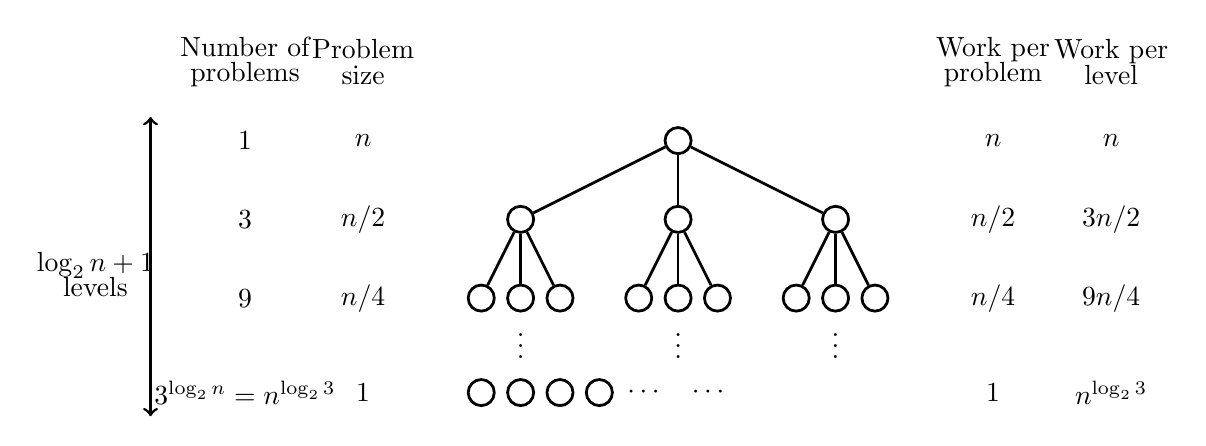
\begin{tikzpicture}[line width = 1pt,
                    solid/.style = {circle, draw, fill = black, minimum size = 0.3cm},
                    empty/.style = {circle, draw, fill = white, minimum size = 0.3cm}]

\draw[<->] (-2.2, 0.3) -- (-2.2, -3.5);
\node at (-2.9, -1.7)[align=center]{$\log_2 n + 1$ \\[-0.1cm] levels};

\node at (-1,1)[align=center]{Number of \\[-0.1cm] problems};
\node at (0.5,1)[align=center]{Problem \\[-0.1cm] size};

% number of problems
\node at (-1,0) {1};
\node at (-1,-1) {3};
\node at (-1,-2) {9};
\node at (-1,-3.2) {$3^{\log_2 n} = n^{\log_2 3}$};

% problem size
\node at (0.5,0) {$n$};
\node at (0.5,-1) {$n/2$};
\node at (0.5,-2) {$n/4$};
\node at (0.5,-3.2) {1};

\node at (8.5,1)[align=center]{Work per \\[-0.1cm] problem};
\node at (10,1)[align=center]{Work per \\[-0.1cm] level};

% work per problem
\node at (8.5,0) {$n$};
\node at (8.5,-1) {$n/2$};
\node at (8.5,-2) {$n/4$};
\node at (8.5,-3.2) {1};

% work per level
\node at (10,0) {$n$};
\node at (10,-1) {$3n/2$};
\node at (10,-2) {$9n/4$};
\node at (10,-3.2) {$n^{\log_2 3}$};

\node [empty] (T11) at (4.5,0) {};
\node [empty] (T21) at (2.5,-1) {};
\node [empty] (T22) at (4.5,-1) {};
\node [empty] (T23) at (6.5,-1) {};
\node [empty] (T31) at (2,-2) {};
\node [empty] (T32) at (2.5,-2) {};
\node [empty] (T33) at (3,-2) {};
\node [empty] (T34) at (4,-2) {};
\node [empty] (T35) at (4.5,-2) {};
\node [empty] (T36) at (5,-2) {};
\node [empty] (T37) at (6,-2) {};
\node [empty] (T38) at (6.5,-2) {};
\node [empty] (T39) at (7,-2) {};

\node at (2.5, -2.5) {$\vdots$};
\node at (4.5, -2.5) {$\vdots$};
\node at (6.5, -2.5) {$\vdots$};

\node [empty] at (2,-3.2) {};
\node [empty] at (2.5,-3.2) {};
\node [empty] at (3,-3.2) {};
\node [empty] at (3.5,-3.2) {};
\node at (4.5, -3.2) {$\cdots \quad \cdots$};

\draw (T11)--(T21);
\draw (T11)--(T22);
\draw (T11)--(T23);
\draw (T21)--(T31);
\draw (T21)--(T32);
\draw (T21)--(T33);
\draw (T22)--(T34);
\draw (T22)--(T35);
\draw (T22)--(T36);
\draw (T23)--(T37);
\draw (T23)--(T38);
\draw (T23)--(T39);

\end{tikzpicture}\par
\normalsize
For the $i$-th level, the total work is $(3/2)^{i-1} n$. Summing over the levels, we get
\begin{align*}
  T(n) &= \sum_{i=1}^{\log_2 n + 1} (3/2)^{i-1} n \\
  &= n \sum_{i=0}^{\log_2 n } (3/2)^i \\
  &= n \frac{(3/2)^{\log_2 n + 1} - 1} {(3/2)-1} \\
  &= n^{\log_2 3}- 2n \\
  &= \Theta(n^{\log_2 3})
\end{align*}

    \item Recursion tree: \\[0.2cm]
    \scriptsize
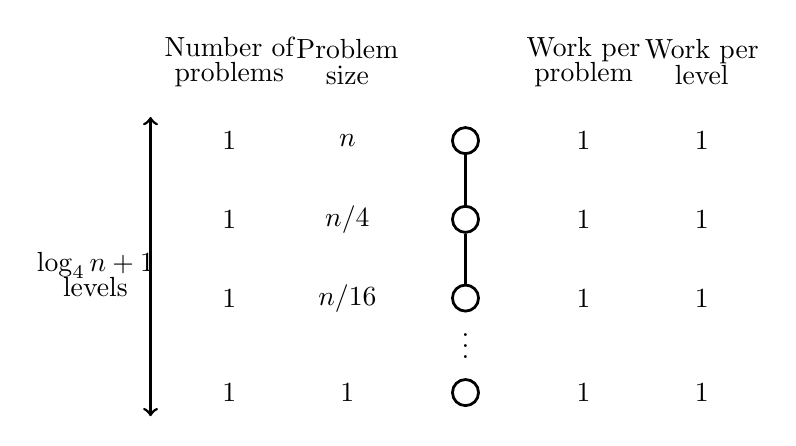
\begin{tikzpicture}[line width = 1pt,
                    solid/.style = {circle, draw, fill = black, minimum size = 0.3cm},
                    empty/.style = {circle, draw, fill = white, minimum size = 0.3cm}]

\draw[<->] (-2, 0.3) -- (-2, -3.5);
\node at (-2.7, -1.7)[align=center]{$\log_4 n + 1$ \\[-0.1cm] levels};

\node at (-1,1)[align=center]{Number of \\[-0.1cm] problems};
\node at (0.5,1)[align=center]{Problem \\[-0.1cm] size};

% number of problems
\node at (-1,0) {1};
\node at (-1,-1) {1};
\node at (-1,-2) {1};
\node at (-1,-3.2) {1};

% problem size
\node at (0.5,0) {$n$};
\node at (0.5,-1) {$n/4$};
\node at (0.5,-2) {$n/16$};
\node at (0.5,-3.2) {1};

\node at (3.5,1)[align=center]{Work per \\[-0.1cm] problem};
\node at (5,1)[align=center]{Work per \\[-0.1cm] level};

% work per problem
\node at (3.5,0) {1};
\node at (3.5,-1) {1};
\node at (3.5,-2) {1};
\node at (3.5,-3.2) {1};

% work per level
\node at (5,0) {1};
\node at (5,-1) {1};
\node at (5,-2) {1};
\node at (5,-3.2) {1};

\node [empty] (T11) at (2,0) {};
\node [empty] (T21) at (2,-1) {};
\node [empty] (T31) at (2,-2) {};
\node at (2, -2.5) {$\vdots$};
\node [empty] at (2,-3.2) {};

\draw (T11)--(T21);
\draw (T21)--(T31);
\end{tikzpicture}\par
\normalsize
For every level, the total work is 1, and there are ($\log_4 n +1$) levels in total, therefore
$$ T(n) = \log_4 n +1 = \Theta(\log n) $$

    \item Recursion tree: \\[0.2cm]
    \scriptsize
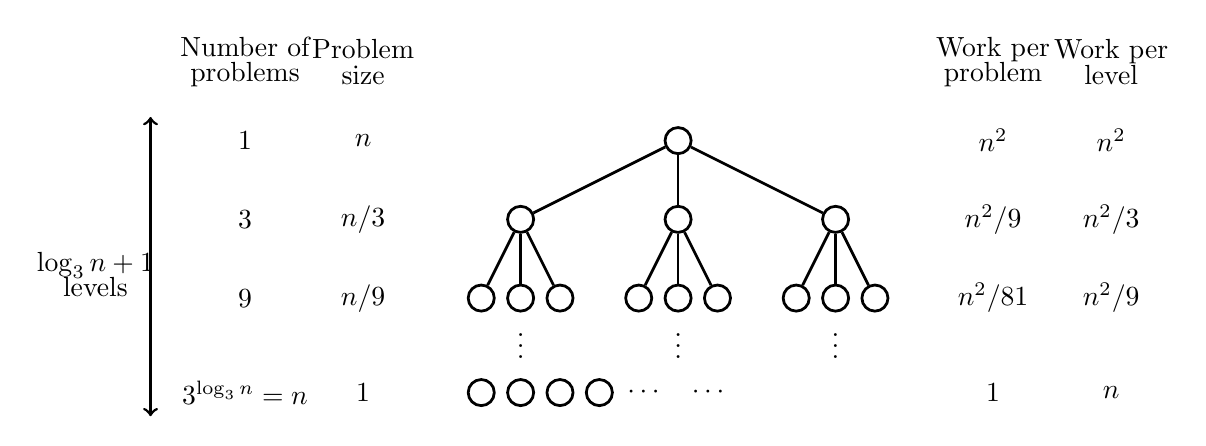
\begin{tikzpicture}[line width = 1pt,
                    solid/.style = {circle, draw, fill = black, minimum size = 0.3cm},
                    empty/.style = {circle, draw, fill = white, minimum size = 0.3cm}]

\draw[<->] (-2.2, 0.3) -- (-2.2, -3.5);
\node at (-2.9, -1.7)[align=center]{$\log_3 n + 1$ \\[-0.1cm] levels};

\node at (-1,1)[align=center]{Number of \\[-0.1cm] problems};
\node at (0.5,1)[align=center]{Problem \\[-0.1cm] size};

% number of problems
\node at (-1,0) {1};
\node at (-1,-1) {3};
\node at (-1,-2) {9};
\node at (-1,-3.2) {$3^{\log_3 n} = n$};

% problem size
\node at (0.5,0) {$n$};
\node at (0.5,-1) {$n/3$};
\node at (0.5,-2) {$n/9$};
\node at (0.5,-3.2) {1};

\node at (8.5,1)[align=center]{Work per \\[-0.1cm] problem};
\node at (10,1)[align=center]{Work per \\[-0.1cm] level};

% work per problem
\node at (8.5,0) {$n^2$};
\node at (8.5,-1) {$n^2/9$};
\node at (8.5,-2) {$n^2/81$};
\node at (8.5,-3.2) {1};

% work per level
\node at (10,0) {$n^2$};
\node at (10,-1) {$n^2/3$};
\node at (10,-2) {$n^2/9$};
\node at (10,-3.2) {$n$};

\node [empty] (T11) at (4.5,0) {};
\node [empty] (T21) at (2.5,-1) {};
\node [empty] (T22) at (4.5,-1) {};
\node [empty] (T23) at (6.5,-1) {};
\node [empty] (T31) at (2,-2) {};
\node [empty] (T32) at (2.5,-2) {};
\node [empty] (T33) at (3,-2) {};
\node [empty] (T34) at (4,-2) {};
\node [empty] (T35) at (4.5,-2) {};
\node [empty] (T36) at (5,-2) {};
\node [empty] (T37) at (6,-2) {};
\node [empty] (T38) at (6.5,-2) {};
\node [empty] (T39) at (7,-2) {};

\node at (2.5, -2.5) {$\vdots$};
\node at (4.5, -2.5) {$\vdots$};
\node at (6.5, -2.5) {$\vdots$};

\node [empty] at (2,-3.2) {};
\node [empty] at (2.5,-3.2) {};
\node [empty] at (3,-3.2) {};
\node [empty] at (3.5,-3.2) {};
\node at (4.5, -3.2) {$\cdots \quad \cdots$};

\draw (T11)--(T21);
\draw (T11)--(T22);
\draw (T11)--(T23);
\draw (T21)--(T31);
\draw (T21)--(T32);
\draw (T21)--(T33);
\draw (T22)--(T34);
\draw (T22)--(T35);
\draw (T22)--(T36);
\draw (T23)--(T37);
\draw (T23)--(T38);
\draw (T23)--(T39);

\end{tikzpicture}\par
\normalsize
For the $i$-th level, the total work is $n^2/3^{i-1}$. Summing over the levels, we get
\begin{align*}
  T(n) &= \sum_{i=1}^{\log_3 n + 1} n^2/3^{i-1} \\
  &= n^2 \sum_{i=0}^{\log_2 n } (1/3)^i \\
  &= \frac{n^2}{2}(3-n^{-\log_2 3}) \\
  &= \Theta(n^2)
\end{align*}
  \end{enumerate}

  \section{[CS] Problem 4.3-13}
  $ a^{\log_b n} = b^{(\log_b a) \log_b n} = b^{(\log_b n) \log_b a} = n^{\log_b a} $

  \section{[CS] Problem 4.3-16}
  Apply Theorem 4.5, we have
  $$ S(n) = a^n S(0) + \sum_{i=1}^n a^{n-i}g(i)$$
  On the one hand, we have
  $$ S(n) \geq a^n S(0)$$
  on the other hand, we have
  \begin{align*}
  S(n) &\leq a^n S(0) + \sum_{i=1}^n a^{n-i} c^i \\
   &= a^n S(0) + a^n \sum_{i=1}^n (c/a)^i  \\
   &\leq a^n S(0) + a^n \frac{c}{a-c} \\
   &= a^n (S(0) + \frac{c}{a-c})
  \end{align*}
  Therefore, $S(n) = \Theta(a^n)$.
  
  \section{[CS] Problem 4.4-1}
  \begin{enumerate}
    \item In this recurrence, we have $a=8$, $b=2$, $d=1$, $f(n)=n=\Theta(n^c)$ where $c=1<\log_b a = 3$. Apply the master theorem, case 3, and we obtain
        $T(n)=\Theta(n^{\log_a b})=\Theta(n^3)$.
    \item In this recurrence, we have $a=8$, $b=2$, $f(n)=n^3=\Theta(n^c)$ where $c=3=\log_b a$. Apply the master theorem, case 2, and we obtain
        $T(n)=\Theta(f(n)\log n)=\Theta(n^3\log n)$.
    \item In this recurrence, we have $a=3$, $b=2$, $f(n)=n=\Theta(n^c)$ where $c=1<\log_b a=\log_2 3$. Apply the master theorem, case 3, and we obtain
        $T(n)=\Theta(n^{\log_a b})=\Theta(n^{\log_2 3})$.
    \item In this recurrence, we have $a=1$, $b=4$, $f(n)=1=\Theta(n^c)$ where $c=0 = \log_b a$. Apply the master theorem, case 2, and we obtain
        $T(n)=\Theta(f(n)\log n)=\Theta(\log n)$.
    \item In this recurrence, we have $a=3$, $b=3$, $f(n)=n^2=\Theta(n^c)$ where $c=2>\log_b a$. Apply the master theorem, case 1, and we obtain
        $T(n)=\Theta(f(n))=\Theta(n^2)$.
  \end{enumerate}
  
  \section{[CS] Problem 4.4-4}
  In this recurrence, $a=3$, $b=2$, $f(n)=\sqrt{n^4+3}=\Theta(n^c)$ where $c=4>\log_b a=\log_2 3$. Apply Theorem 4.11, case 1, and we obtain $T(n)=\Theta(f(n))=\Theta(n^4)$.
  
  \section{[CS] Problem 4.4-6}
  Define $S(n) = T(n)/d$, then 
  $$ S(n) = 
   \begin{cases} 
     aS(n/b) + (n^c)/d & \text{if } n>1 \\
     1 & \text{if } n=1 
   \end{cases} $$
  Apply the master theorem, and we obtain: \par
  1. If $\log_b a < c$, then $T(n) = \Theta((n^c)/d) = \Theta(n^c)$. \par
  2. If $\log_b a = c$, then $T(n) = \Theta(\log n (n^c)/d) = \Theta(n^c \log n)$. \par
  3. If $\log_b a > c$, then $T(n) = \Theta(n^{\log_b a})$.
  
  \section{[CS] Problem 4.5-8}
  To prove $T(n)=O(n^3)$, we have to prove that, there exists some positive constant $k$, such that for every positive integer $n$, $T(n) \leq kn^3 - n \log n$ holds. \par
  For the base step, $n=1$, we have $T(n)=d$, $n^3=1$ and $n \log n=0$, therefore $T(n) \leq kn^3 - n\log n$ holds for every $k>d$ when $n=1$. \par
  For the induction step, assume that $T(m) \leq km^3 - m \log m$ holds for all $m<n$. Substituting into the recurrence yields
  \begin{align*}
    T(n) &= 8T(n/2) + n\log n \\
    &\leq 8(k(n/2)^3 - (n/2) \log (n/2) + n \log n \\
    &= kn^3-4n\log n - 4n \log 2 + n\log n \\
    &\leq kn^3 - n \log n
  \end{align*} \par
  By mathematical induction, we conclude that $T(n) \leq kn^3 - n \log n$ where $k>d$. Hence, $T(n) = O(kn^3 - n\log n) = O(n^3)$.
  
  \section{[CS] Problem 4.5-9}
  Yes. \par
  Define $S(n) = \begin{cases} 
    8S(n/2)+n & \text{if } n>1 \\
    d & \text{if } n=1
  \end{cases}$, it is true that $S(n) \leq T(n)$ because $n < n \log n$ holds for every $n \geq 2$. For $S(n)$, $a=8$, $b=2$, $f(n) = n = n^c$ where $c=1 < \log_2 8 = 3$. Apply the master theorem, case 3, and we obtain $S(n) = \Theta(n^{\log_b a}) = \Theta(n^3)$. Because $S(n) \leq T(n)$, we get $T(n) = \Omega(n^3)$. We have proved that $T(n) = O(n^3)$ in Problem 8, so $T(n) = \Theta(n^3)$.
  
  \section{[CS] Problem 4.5-10}
  $T(n) = O(n)$. \par
  To prove $T(n) = O(n)$, we have to prove that there exists some positive constant $k$, such that $T(n) \leq kn$ holds for every positive integer $n$. \par
  For the base step, we have to prove that $T(n) \leq kn$ holds for every positive integer $n \leq 12 $. This inequality holds if we choose $k > \max\limits_{0<n<12} T(n)/n$. \par
  For the induction step, assume that $T(m) \leq km$ holds for every $m<n$. Substituting into the recurrence yields
  \begin{align*}
    T(n) &= 2T(\frac{n}{3}-3) + n \\
    &\leq 2k(\frac{n}{3}-3) + n \\
    &= \left(\frac{2k}{3}+1\right)n - 6k\\
    &\leq kn
  \end{align*}
  The last step holds if we choose $k>3$. \par
  By mathematical induction, we conclude that $T(n) < kn$ holds for every positive integer if we choose $k > \max\{\max\limits_{0<n<12} T(n)/n, 3\}$. Therefore $T(n) = O(n)$.
  
\end{document}
